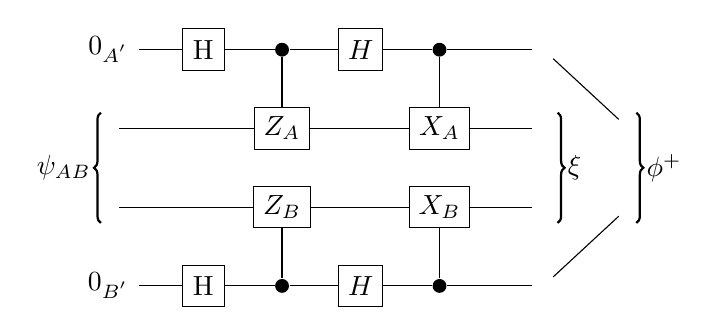
\begin{tikzpicture}
    %
    % `operator' will only be used by Hadamard (H) gates here.
    % `phase' is used for controlled phase gates (dots).
    % `surround' is used for the background box.
    \tikzstyle{operator} = [draw,fill=white,minimum size=1.5em] 
    \tikzstyle{phase} = [fill,shape=circle,minimum size=5pt,inner sep=0pt]
  % \tikzstyle{surround} = [fill=blue!10,thick,draw=black,rounded corners=2mm]
  %
  % Qubits
  \node at (0.3,0) (q1) {$\ket{0}_{A^{'}}$ };
  %\node at (0,-1) (q11) {$\ket{+}^{\rC_i''}$ };
  \node at (0.3,-1) (q2) {};
  \node at (0.3,-2) (q3) {};
  \node at (0.3,-3) (q4) { $\ket{0}_{B^{'}}$};
  \draw[decorate,decoration={brace, mirror},thick] (0.2,-0.8) to 	node[midway,left] (bracket) {$\ket{\psi}_{AB}$} (0.2,-2.2);
    % Column 1
    %\node[phase] (phase11) at (1.5,0) {} edge [-] (q1);
    %\node[operator] (phase12) at (1.5,-1) {${\tilde{\X}}_{1,A}$} edge [-] (q2);
    %\draw[-] (phase11) -- (phase12);
    %\node[phase] (phase13) at (1.5,-3) {} edge [-] (q4);
    %\node[operator] (phase14) at (1.5,-2) {${\tilde{\X}}_{1,B}$} edge [-] (q3);
    %\draw[-] (phase13) -- (phase14);
    % Column 2
    \node[operator] (op12) at (1.5,0) {H} edge [-] (q1);
    \node[operator] (op22) at (1.5,-3) {H} edge [-] (q4);
    %
 % Column 3
    \node[phase] (phase21) at (2.5,0) {} edge [-] (op12);
    \node[operator] (phase22) at (2.5,-1) {$Z_A$} edge [-] (q2);
    \draw[-] (phase21) -- (phase22);
    \node[phase] (phase23) at (2.5,-3) {} edge [-] (op22);
    \node[operator] (phase24) at (2.5,-2) {$Z_B$} edge [-] (q3);
    \draw[-] (phase23) -- (phase24);
     % Column 4
    \node[operator] (op14) at (3.5,0) {$H$} edge [-] (phase21);
    \node[operator] (op24) at (3.5,-3) {$H$} edge [-] (phase23);
    %  
 % Column 5
    \node[phase] (phase31) at (4.5,0) {} edge [-] (op14);
    \node[operator] (phase32) at (4.5,-1) {$X_A$} edge [-] (phase22);
    \draw[-] (phase31) -- (phase32);
    \node[phase] (phase33) at (4.5,-3) {} edge [-] (op24);
    \node[operator] (phase34) at (4.5,-2) {$X_B$} edge [-] (phase24);
    \draw[-] (phase33) -- (phase34);
%
    \node (end1) at (5.8,0) {} edge [-] (phase31);
    %\node (end5) at (9,-1) {} edge [-] (op81); 
    \node (end2) at (5.8,-1) {} edge [-] (phase32);
    \node (end3) at (5.8,-2) {} edge [-] (phase34);
    %\node (end6) at (9,-4) {} edge [-] (op82);
    \node (end4) at (5.8,-3) {} edge [-] (phase33);
    %
    % Bracket
    \draw[decorate,decoration={brace},thick] (6,-0.8) to 	node[midway,right] (bracket) {$\ket{\xi}$} (6,-2.2);
    \node at (5.82,0) (eend1) {};
    \node at (6.9,-1) (eend11) {};
    \draw[-] (eend1) -- (eend11);
    \node at (5.82,-3) (eend4) {};
    \node at (6.9,-2) (eend44) {};
    \draw[-] (eend4) -- (eend44);
    \draw[decorate,decoration={brace},thick] (7,-0.8) to 	node[right] (bracket) {$\ket{\phi^{+}}$} 	(7,-2.2);
    %
    % Background Box
  %  \begin{pgfonlayer}{background} 
  % \node[surround] (background) [fit = (q1) (op31) (bracket)] {};
  %  \end{pgfonlayer}
    %
\end{tikzpicture}